\section{Arduino Sensor Gas}
\subsection{Pengertian Arduino}
Arduino adalah perusahaan perangkat keras dan perangkat lunak komputer open-source, proyek, dan komunitas pengguna yang merancang dan memproduksi mikrokontroler board tunggal dan kit mikrokontroler untuk membangun perangkat digital dan objek interaktif yang dapat merasakan dan mengendalikan objek di dunia fisik.
Produk proyek didistribusikan sebagai perangkat keras dan perangkat lunak open-source, yang berlisensi di bawah GNU Lesser General Public License (LGPL) atau GNU General Public License (GPL), yang mengizinkan pembuatan papan Arduino dan distribusi perangkat lunak oleh siapa saja. Papan Arduino tersedia secara komersil dalam bentuk preassembled, atau sebagai kit do-it-yourself (DIY)\cite{kushner2011making}
\subsection{sensor gas}
Sensor yang digunakan kali ini adalah sensor MQ-2, sensor ini digunakan untuk mendeteksi gas LPG, i-butana, propana, alkohol, hidroge, dan asap. Inti dari MQ-2 adalah material yang sensitif terhadap konsentrasi gas yang tersusun dari senyawa SnO2 atau Timah Oksida. Material ini mempunyai karakteristik yang akan merubah konduktivitasnya seiring dengan perubahan konsenterasi gas.
Sedangkan untuk spesifikasi sensor MQ-2, adalah:
\begin{itemize}
\item suhu 20 derajat Celcius
\item kelembaban udara 65 persen
\end{itemize}
range konsentrasi gas yang bisa diukur:
\begin{itemize}
\item LPG dan propana: 200ppm-5000ppm
\item butana: 300ppm-5000ppm
\item metana: 5000ppm - 20000ppm
\end{itemize}

\subsection{hardware yang digunakan}
Perangkat Keras Sistem pengukuran kami terdiri dari beberapa bagian. Kami menggunakan modul sensor MQ-2 untuk merasakan gas. Komunikasi digital dimungkinkan melalui antarmuka RS232 board. Arduino Uno board terhubung ke modul sensor gas MQ2 dan terhubung melalui USB ke sistem komputer untuk mencatat data real-time dari sensor. Semua bagian praktikum ini termasuk modul sensor dan arduino mudah didapat dengan harga murah. Hal ini penting untuk mendapatkan penerimaan yang luas terhadap sistem pemantauan asap.
	
\subsection{Koneksi Sensor Modul}
Sambungan modul sensor Modul sensor gas MQ2 terhubung ke papan Arduino menggunakan kabel jumper. Pin Analog pada sensor terhubung ke pin analog 0 pada papan arduino, sedangkan pin + 5 V dan GND pada modul sensor terhubung ke pin 5V Vcc dan GND (ground) masing-masing pada papan arduino. Arduino Uno board kemudian dihubungkan ke sistem komputer dengan menggunakan koneksi USB dan antarmuka RS232.

\subsection{Eksperimen}
Alat dan bahan:
\begin{enumerate}
\item Arduino Uno
\item Sensor MQ
\item Led
\end{enumerate}
Kode
\begin{verbatim}
int redLed = 12;
int redLed = 11;
int redLed = 10;
int smokeA0 = A5;
// Your threshold value
int sensorThres = 400;

void setup() {
  pinMode(redLed, OUTPUT);
  pinMode(redLed, OUTPUT);
  pinMode(redLed, OUTPUT);
   pinMode(smokeA0, INPUT);
  Serial.begin(9600);
}

void loop() {
  int analogSensor = analogRead(smokeA0);

  Serial.print("Pin A0: ");
  Serial.println(analogSensor);
  // Checks if it has reached the threshold value
  if (analogSensor > sensorThres)
  {
    digitalWrite(redLed, HIGH);
    digitalWrite(redLed, LOW);
    digitalWrite(redLed, HIGH);
  }
  else
  {
    digitalWrite(redLed, LOW);
    digitalWrite(redLed, HIGH);
    digitalWrite(redLed, LOW);
  }
  delay(100);
}
\end{verbatim}

Keadaan sensor jika mendeteksi gas ada pada gambar \ref{terditeksi} dua lampu akan menyala, sedangkan jika tidak, dua lampu akan padam seperti pada gambar \ref{tidakterditeksi}

\begin{figure}[ht]
	\centerline{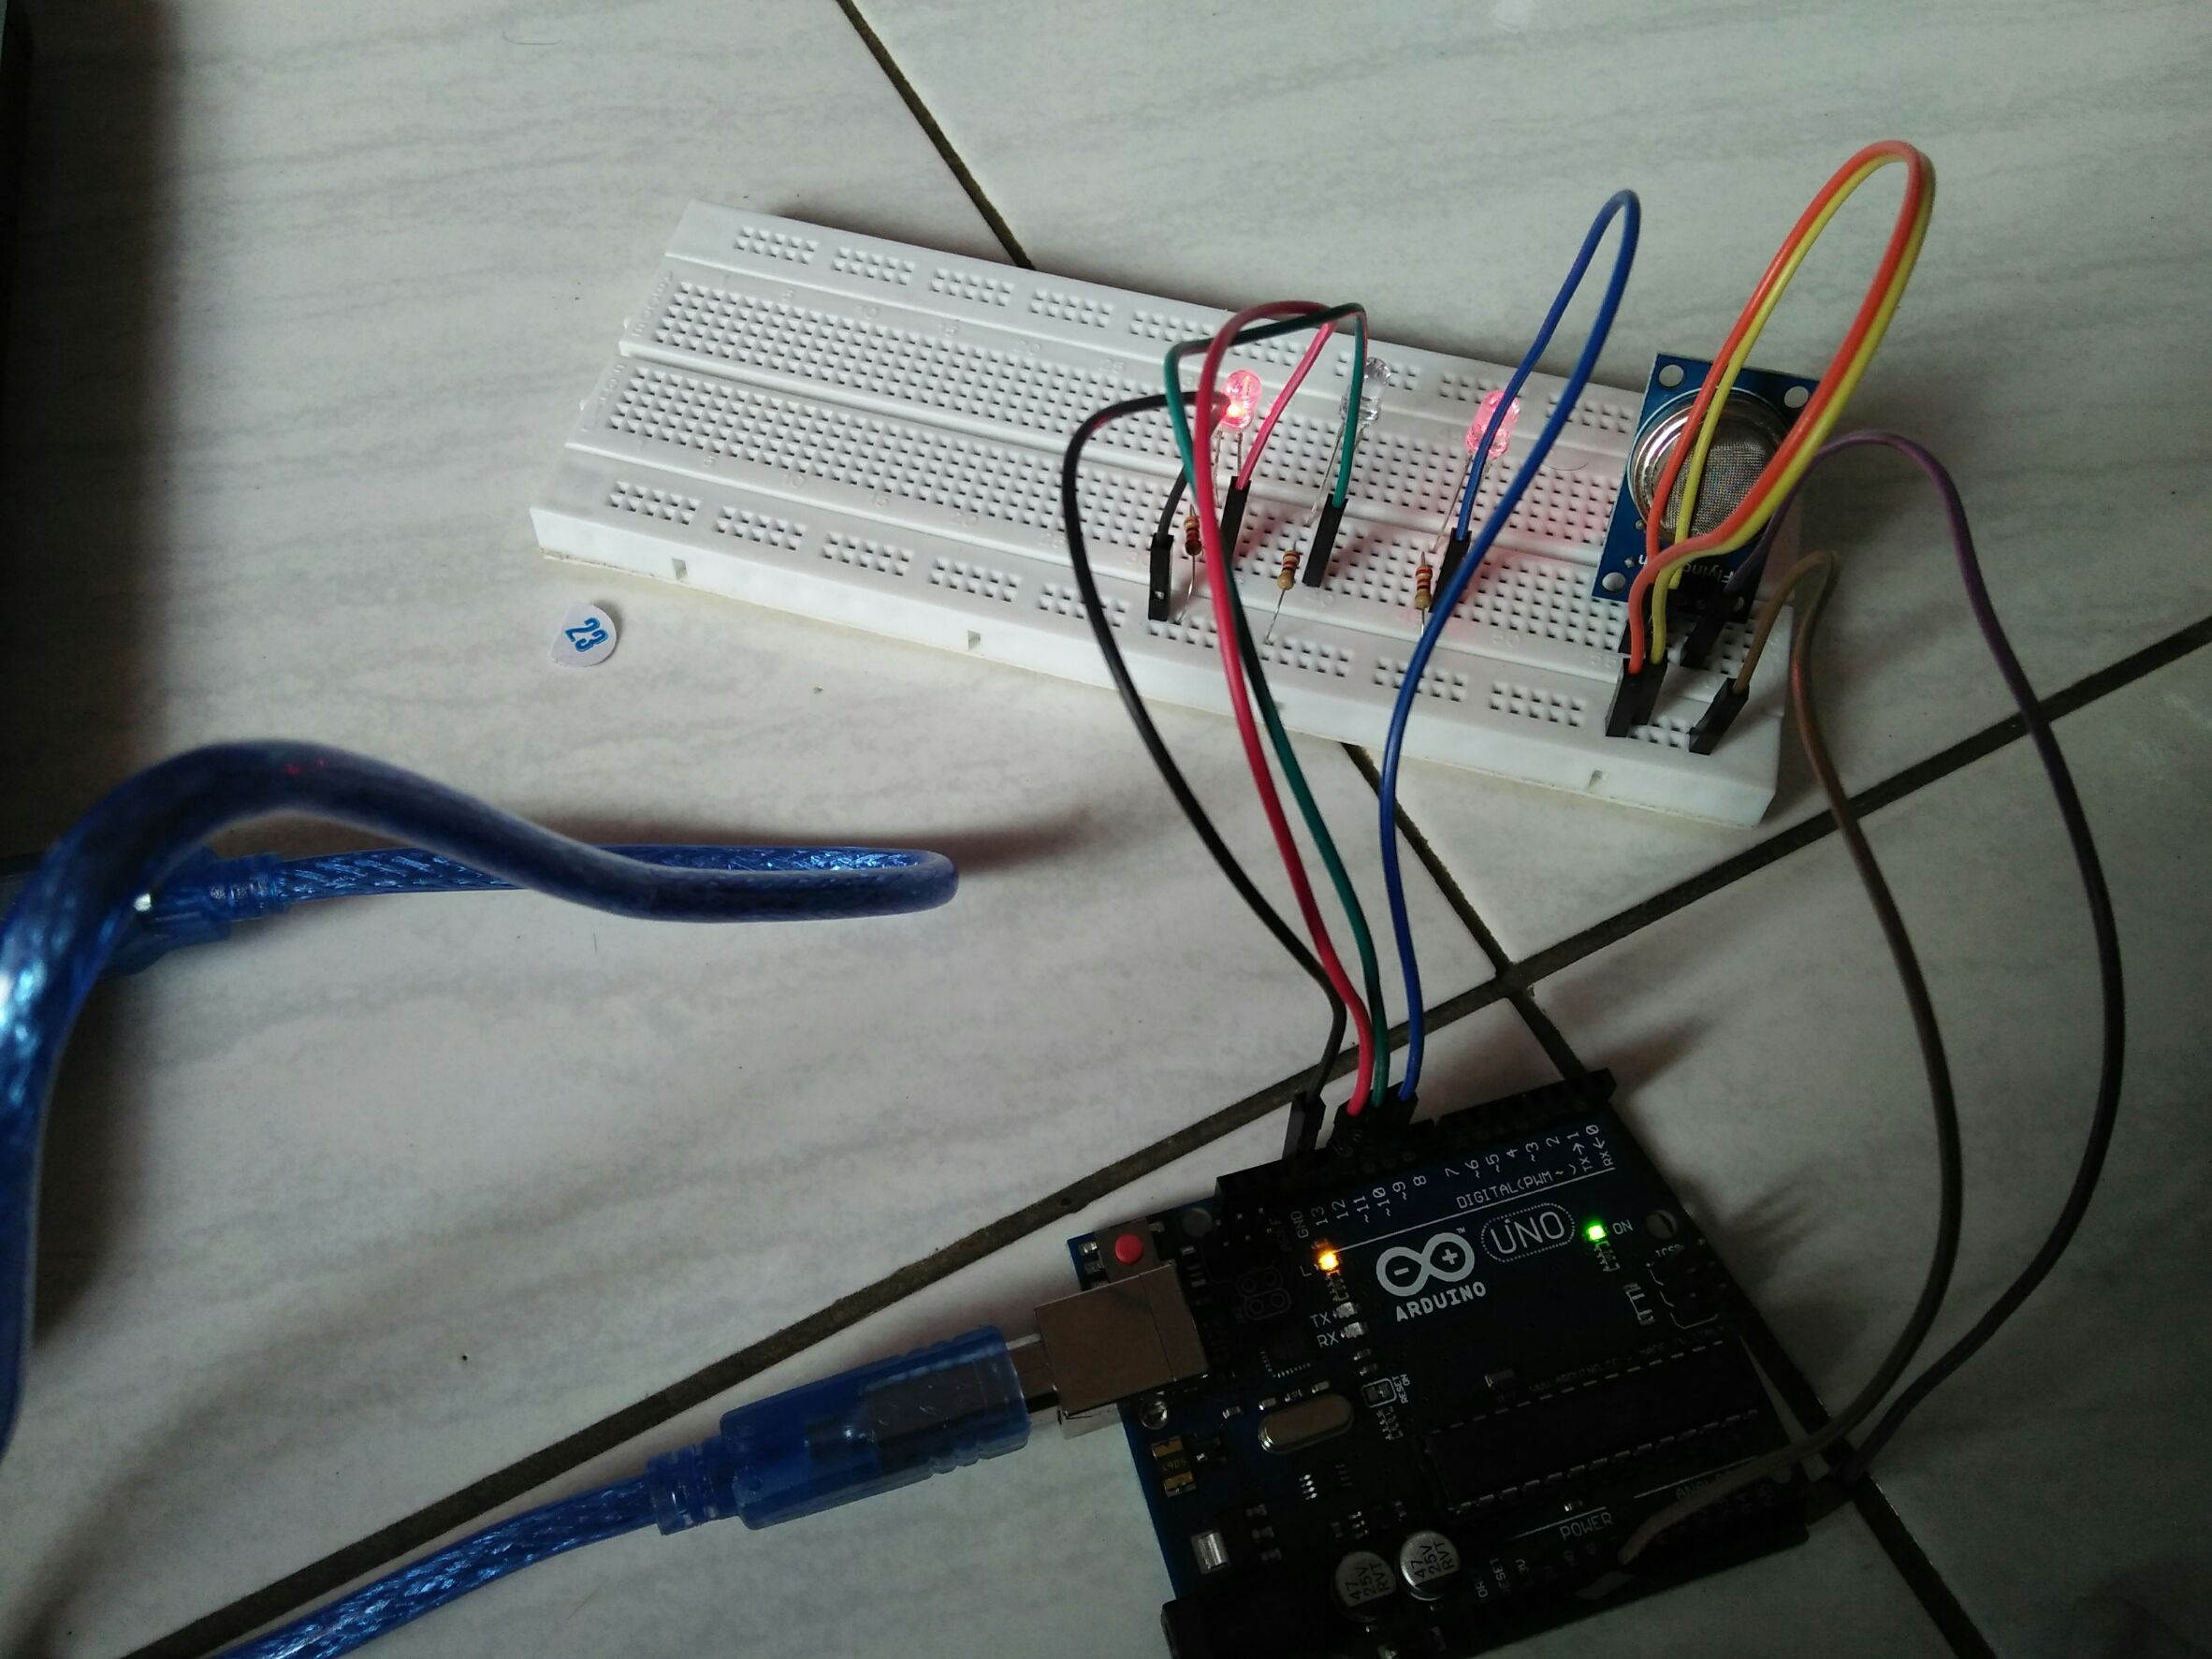
\includegraphics[width=1\textwidth]{figures/terditeksi.jpg}}
	\caption{dua lampu menyala tanda sensor menditeksi gas.}
	\label{terditeksi}
	\end{figure}
\begin{figure}[ht]
	\centerline{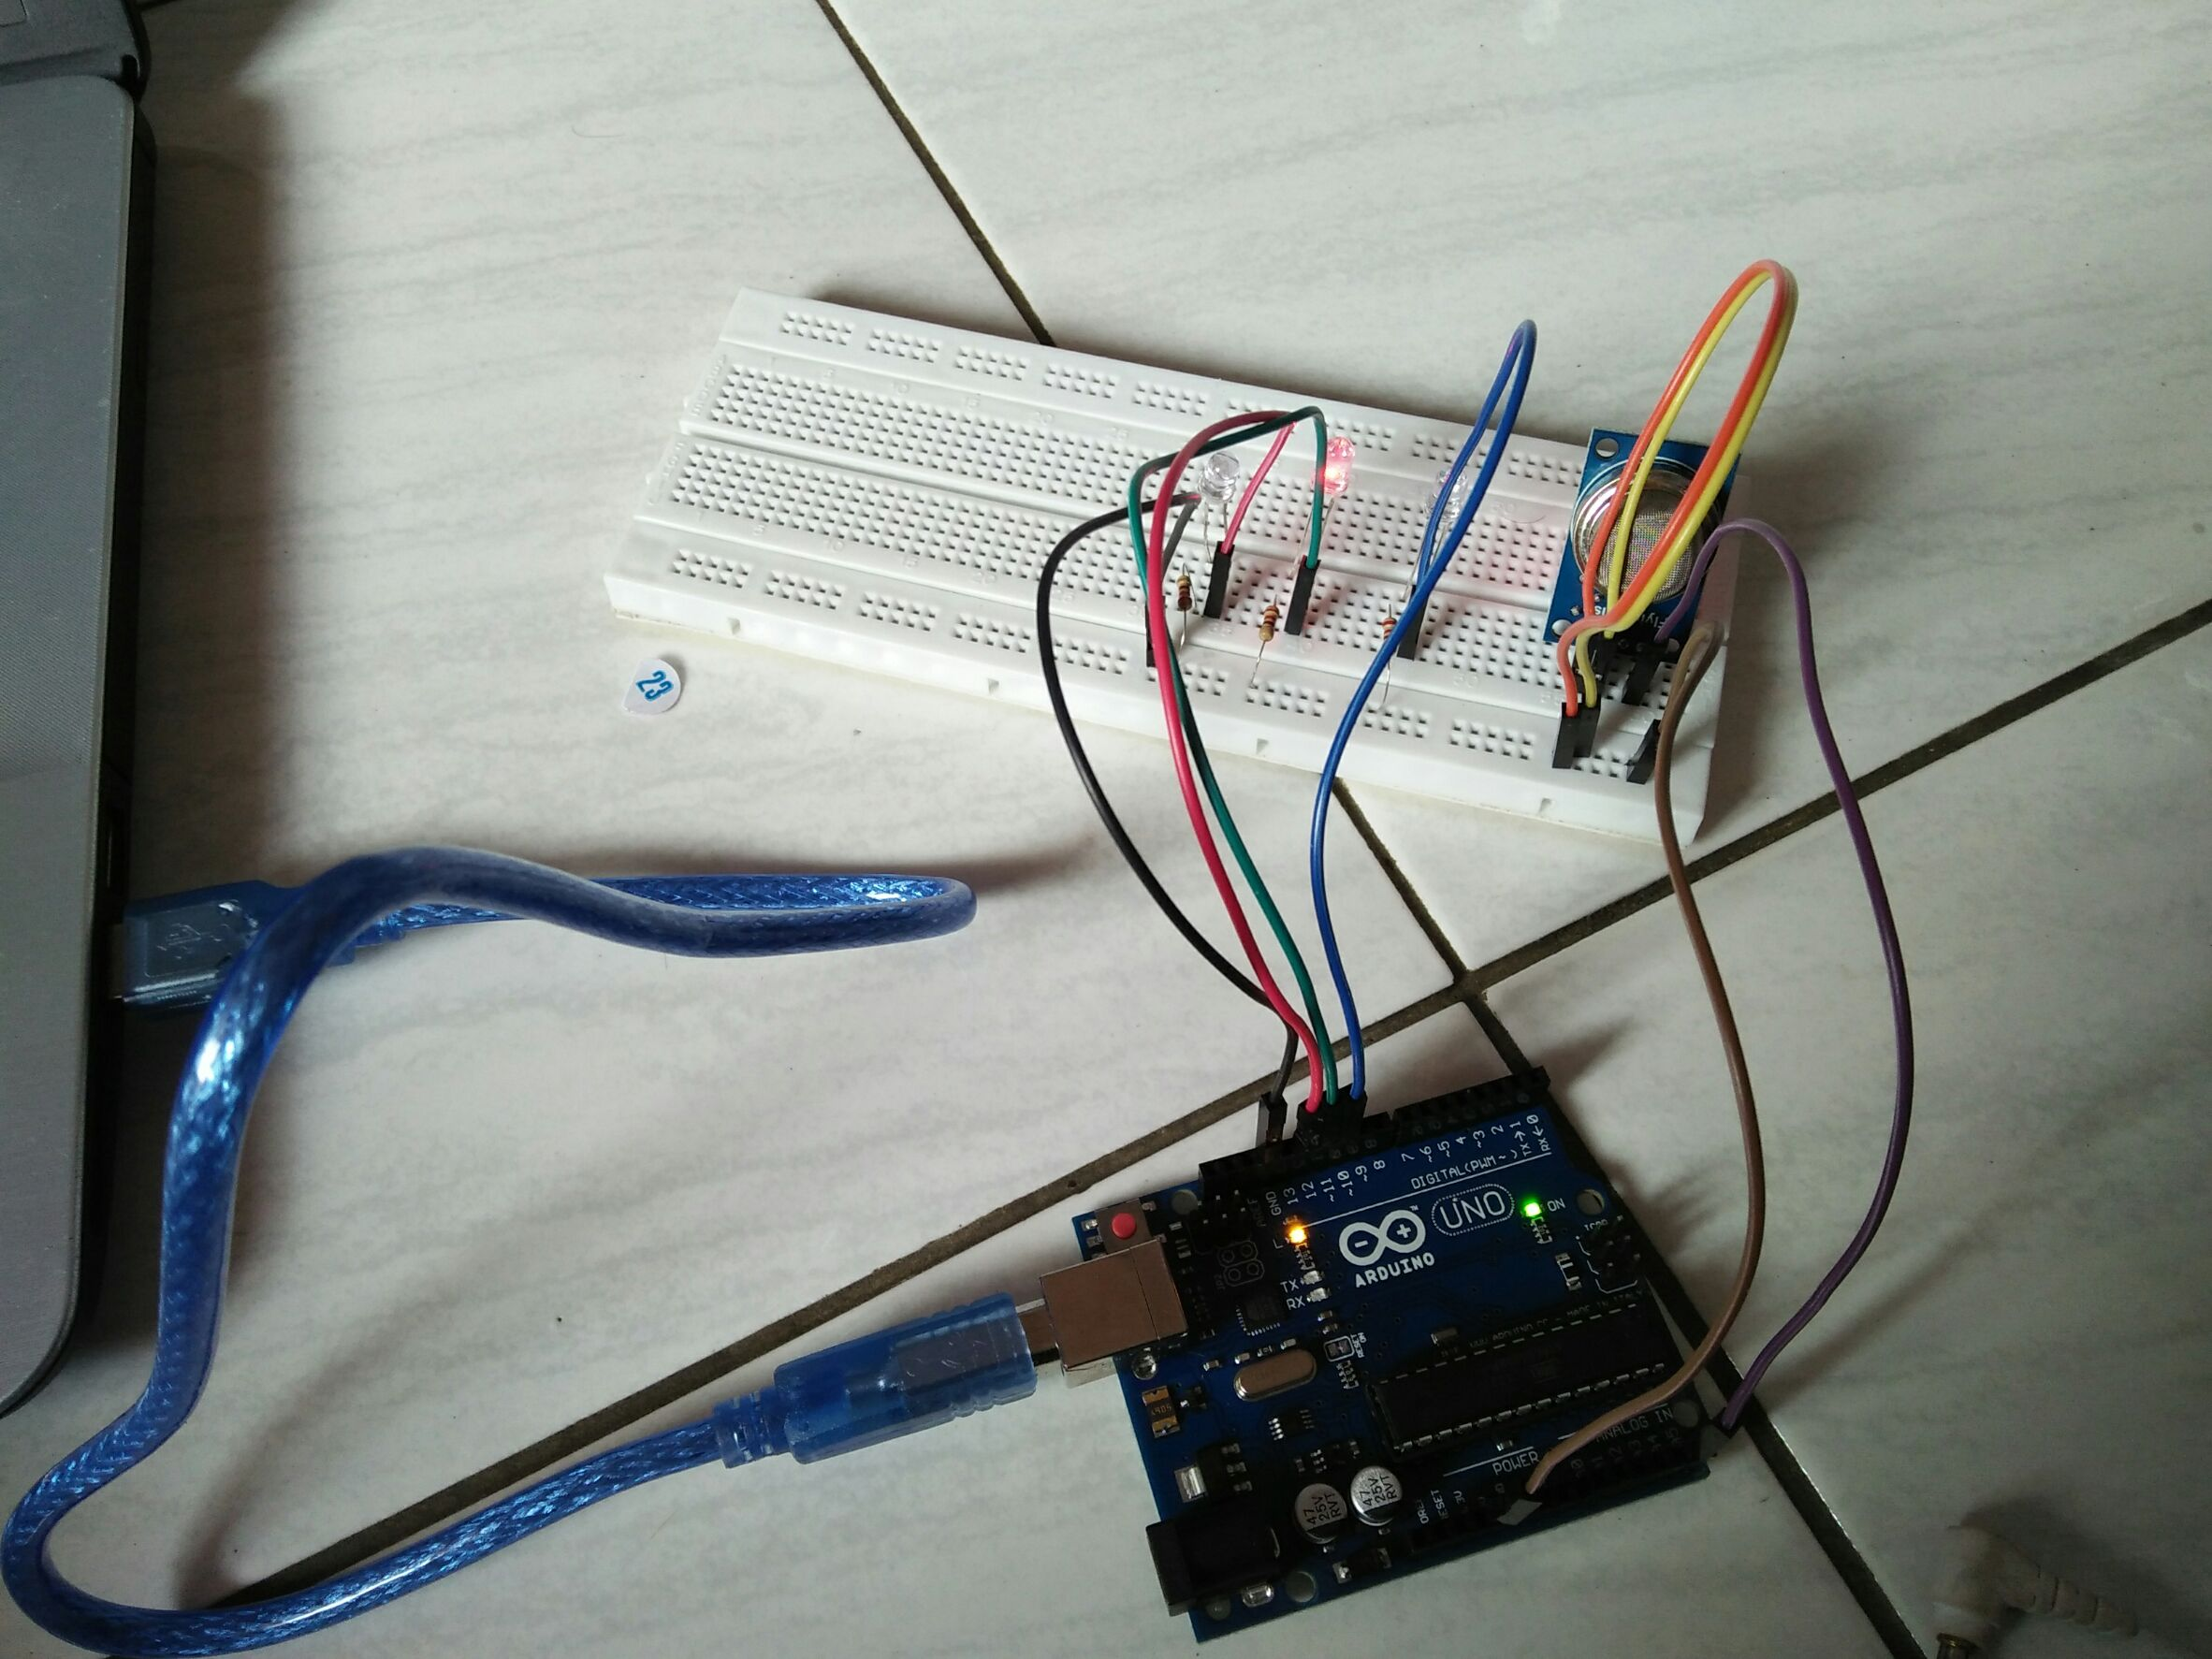
\includegraphics[width=1\textwidth]{figures/tidakterditeksi.jpg}}
	\caption{satu lampu menyala tanda sensor tidak menditeksi gas.}
	\label{tidakterditeksi}
	\end{figure}
	
Setelah Codingan Berhasil di jalankan maka akan munjul Serial Monitor seperti gambar  \ref{SerialMonitor}
\begin{figure}[ht]
	\centerline{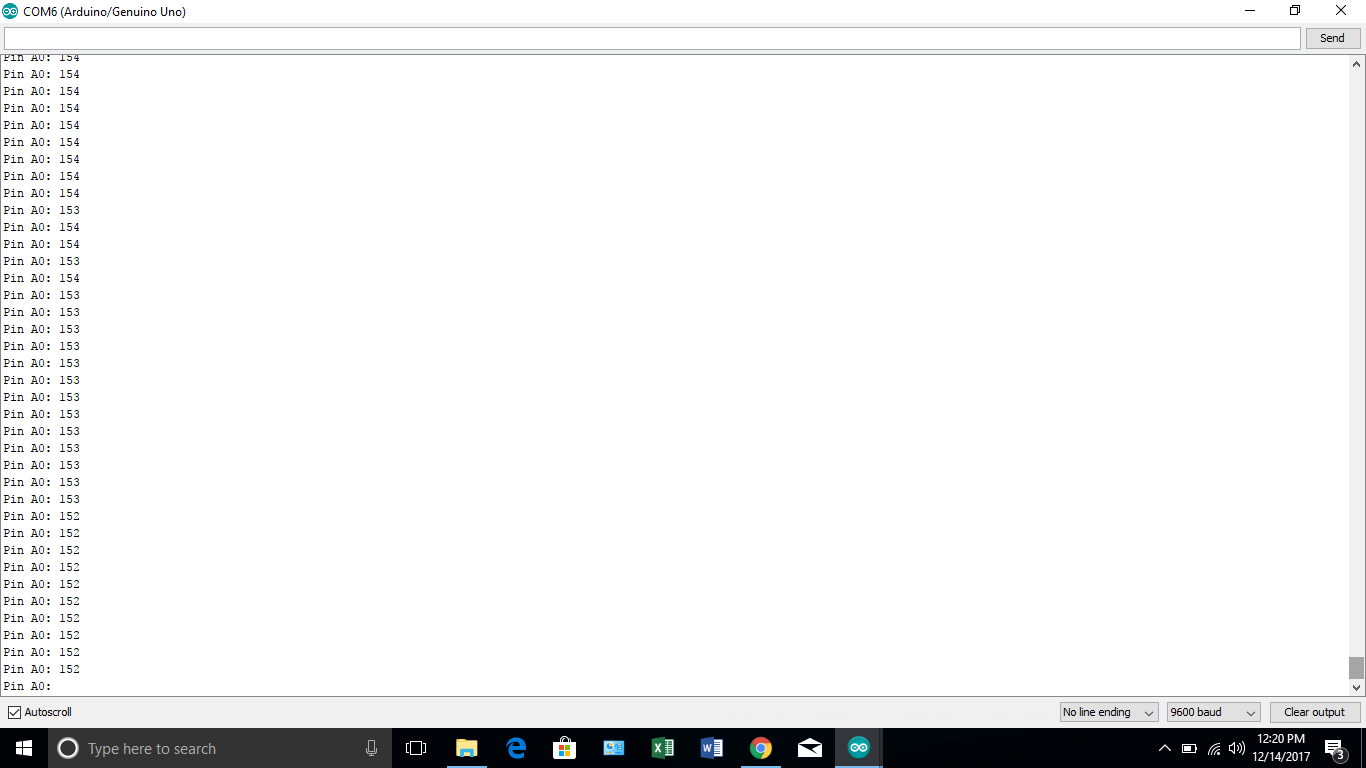
\includegraphics[width=1\textwidth]{figures/SerialMonitor.png}}
	\caption{Serial Monitor Pada Sensor Gas}
	\label{SerialMonitor}
	\end{figure}
